%% fig_vgcounts.tex   (generated by make_round41.py; do not edit by hand)
%% Hodge classes of degree r on the very general member against h^{r/2,r/2} (thm:vgvandermonde(iii)).
\documentclass[tikz,border=8pt]{standalone}
\usepackage{amsmath,amssymb}
\usetikzlibrary{arrows.meta,calc,decorations.pathreplacing}
%% palette.tex -- shared colour definitions for the figures
\definecolor{PInk}{RGB}{26,32,44}
\definecolor{PBlue}{RGB}{37,82,139}
\definecolor{PTeal}{RGB}{23,127,125}
\definecolor{POchre}{RGB}{193,138,44}
\definecolor{PClay}{RGB}{178,74,58}
\definecolor{PSlate}{RGB}{108,122,137}
\definecolor{PViolet}{RGB}{110,86,150}
\definecolor{WBlue}{RGB}{223,234,246}
\definecolor{WTeal}{RGB}{220,238,236}
\definecolor{WOchre}{RGB}{250,240,218}
\definecolor{WClay}{RGB}{247,229,224}
\definecolor{WSlate}{RGB}{238,241,244}
\definecolor{PMag}{RGB}{158,58,110}
\definecolor{PGrass}{RGB}{62,124,66}
\definecolor{PAmber}{RGB}{214,112,38}
\definecolor{PIndigo}{RGB}{58,64,140}
\definecolor{PRule}{RGB}{176,186,197}

%% shared macros so the standalone figures match the paper
\providecommand{\QQ}{\mathbb{Q}}
\providecommand{\ZZ}{\mathbb{Z}}
\providecommand{\RR}{\mathbb{R}}
\providecommand{\CC}{\mathbb{C}}
\providecommand{\PP}{\mathbb{P}}
\providecommand{\Kx}{K^{\times}}
\providecommand{\HW}{W}
\providecommand{\Nm}{\mathrm{N}}
\providecommand{\Hdg}{\mathrm{Hdg}}
\providecommand{\NS}{\mathrm{NS}}
\providecommand{\cA}{\mathcal{A}}
\providecommand{\cD}{\mathcal{D}}
\providecommand{\cF}{\mathcal{F}}
\providecommand{\cP}{\mathcal{P}}
\providecommand{\cO}{\mathcal{O}}
\providecommand{\cQ}{\mathcal{Q}}
\providecommand{\bbar}[1]{\overline{#1}}
\providecommand{\ch}{\operatorname{ch}}
\providecommand{\End}{\mathrm{End}}
\providecommand{\Ext}{\operatorname{Ext}}
\providecommand{\Supp}{\operatorname{Supp}}

\begin{document}
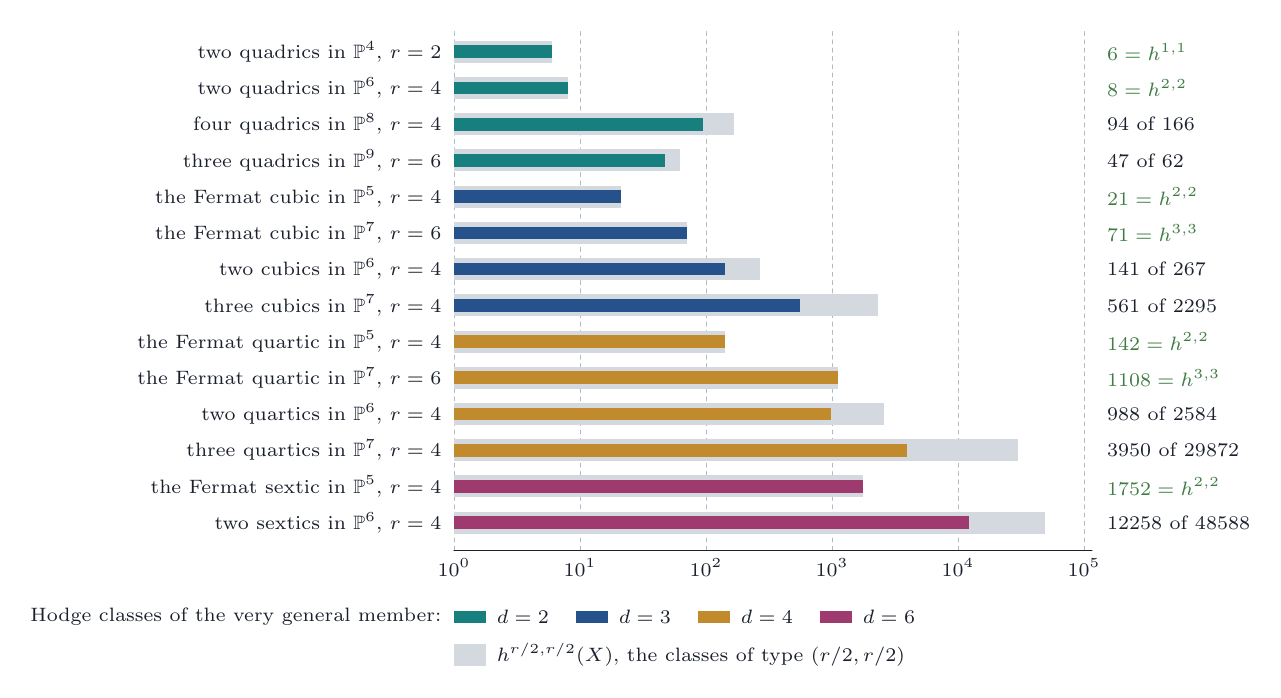
\begin{tikzpicture}[x=1cm,y=1cm,line join=round,line cap=round,
  font=\small,text=PInk,lbl/.style={inner sep=1pt}]
  \draw[PRule,line width=0.35pt,dash pattern=on 1.4pt off 1.6pt] (5.6000,-0.3500) -- (5.6000,6.2800);
  \draw[PRule,line width=0.35pt,dash pattern=on 1.4pt off 1.6pt] (7.2000,-0.3500) -- (7.2000,6.2800);
  \draw[PRule,line width=0.35pt,dash pattern=on 1.4pt off 1.6pt] (8.8000,-0.3500) -- (8.8000,6.2800);
  \draw[PRule,line width=0.35pt,dash pattern=on 1.4pt off 1.6pt] (10.4000,-0.3500) -- (10.4000,6.2800);
  \draw[PRule,line width=0.35pt,dash pattern=on 1.4pt off 1.6pt] (12.0000,-0.3500) -- (12.0000,6.2800);
  \draw[PRule,line width=0.35pt,dash pattern=on 1.4pt off 1.6pt] (13.6000,-0.3500) -- (13.6000,6.2800);
  \draw[PInk,line width=0.5pt] (5.6000,-0.3500) -- (13.7000,-0.3500);
  \path[fill=PRule!55!white,draw=none] (5.6000,5.8400) rectangle (6.8450,6.1200);
  \path[fill=PTeal,draw=none] (5.6000,5.9000) rectangle (6.8450,6.0600);
  \path[fill=PRule!55!white,draw=none] (5.6000,5.3800) rectangle (7.0449,5.6600);
  \path[fill=PTeal,draw=none] (5.6000,5.4400) rectangle (7.0449,5.6000);
  \path[fill=PRule!55!white,draw=none] (5.6000,4.9200) rectangle (9.1522,5.2000);
  \path[fill=PTeal,draw=none] (5.6000,4.9800) rectangle (8.7570,5.1400);
  \path[fill=PRule!55!white,draw=none] (5.6000,4.4600) rectangle (8.4678,4.7400);
  \path[fill=PTeal,draw=none] (5.6000,4.5200) rectangle (8.2754,4.6800);
  \path[fill=PRule!55!white,draw=none] (5.6000,4.0000) rectangle (7.7156,4.2800);
  \path[fill=PBlue,draw=none] (5.6000,4.0600) rectangle (7.7156,4.2200);
  \path[fill=PRule!55!white,draw=none] (5.6000,3.5400) rectangle (8.5620,3.8200);
  \path[fill=PBlue,draw=none] (5.6000,3.6000) rectangle (8.5620,3.7600);
  \path[fill=PRule!55!white,draw=none] (5.6000,3.0800) rectangle (9.4824,3.3600);
  \path[fill=PBlue,draw=none] (5.6000,3.1400) rectangle (9.0388,3.3000);
  \path[fill=PRule!55!white,draw=none] (5.6000,2.6200) rectangle (10.9773,2.9000);
  \path[fill=PBlue,draw=none] (5.6000,2.6800) rectangle (9.9983,2.8400);
  \path[fill=PRule!55!white,draw=none] (5.6000,2.1600) rectangle (9.0437,2.4400);
  \path[fill=POchre,draw=none] (5.6000,2.2200) rectangle (9.0437,2.3800);
  \path[fill=PRule!55!white,draw=none] (5.6000,1.7000) rectangle (10.4713,1.9800);
  \path[fill=POchre,draw=none] (5.6000,1.7600) rectangle (10.4713,1.9200);
  \path[fill=PRule!55!white,draw=none] (5.6000,1.2400) rectangle (11.0597,1.5200);
  \path[fill=POchre,draw=none] (5.6000,1.3000) rectangle (10.3916,1.4600);
  \path[fill=PRule!55!white,draw=none] (5.6000,0.7800) rectangle (12.7604,1.0600);
  \path[fill=POchre,draw=none] (5.6000,0.8400) rectangle (11.3546,1.0000);
  \path[fill=PRule!55!white,draw=none] (5.6000,0.3200) rectangle (10.7897,0.6000);
  \path[fill=PMag,draw=none] (5.6000,0.3800) rectangle (10.7897,0.5400);
  \path[fill=PRule!55!white,draw=none] (5.6000,-0.1400) rectangle (13.0984,0.1400);
  \path[fill=PMag,draw=none] (5.6000,-0.0800) rectangle (12.1415,0.0800);
  \path[fill=PTeal,draw=none] (5.6000,-1.2800) rectangle (6.0000,-1.1200);
  \path[fill=PBlue,draw=none] (7.1500,-1.2800) rectangle (7.5500,-1.1200);
  \path[fill=POchre,draw=none] (8.7000,-1.2800) rectangle (9.1000,-1.1200);
  \path[fill=PMag,draw=none] (10.2500,-1.2800) rectangle (10.6500,-1.1200);
  \path[fill=PRule!55!white,draw=none] (5.6000,-1.8200) rectangle (6.0000,-1.5400);
  \node[lbl,anchor=north,text=PInk,font=\scriptsize] at (5.6000,-0.4200) {$10^{0}$};
  \node[lbl,anchor=north,text=PInk,font=\scriptsize] at (7.2000,-0.4200) {$10^{1}$};
  \node[lbl,anchor=north,text=PInk,font=\scriptsize] at (8.8000,-0.4200) {$10^{2}$};
  \node[lbl,anchor=north,text=PInk,font=\scriptsize] at (10.4000,-0.4200) {$10^{3}$};
  \node[lbl,anchor=north,text=PInk,font=\scriptsize] at (12.0000,-0.4200) {$10^{4}$};
  \node[lbl,anchor=north,text=PInk,font=\scriptsize] at (13.6000,-0.4200) {$10^{5}$};
  \node[lbl,anchor=east,text=PInk,font=\scriptsize] at (5.4800,5.9800) {two quadrics in $\PP^{4}$, $r=2$};
  \node[lbl,anchor=west,text=PGrass,font=\scriptsize] at (13.8500,5.9800) {$6=h^{1,1}$};
  \node[lbl,anchor=east,text=PInk,font=\scriptsize] at (5.4800,5.5200) {two quadrics in $\PP^{6}$, $r=4$};
  \node[lbl,anchor=west,text=PGrass,font=\scriptsize] at (13.8500,5.5200) {$8=h^{2,2}$};
  \node[lbl,anchor=east,text=PInk,font=\scriptsize] at (5.4800,5.0600) {four quadrics in $\PP^{8}$, $r=4$};
  \node[lbl,anchor=west,text=PInk,font=\scriptsize] at (13.8500,5.0600) {$94$ of $166$};
  \node[lbl,anchor=east,text=PInk,font=\scriptsize] at (5.4800,4.6000) {three quadrics in $\PP^{9}$, $r=6$};
  \node[lbl,anchor=west,text=PInk,font=\scriptsize] at (13.8500,4.6000) {$47$ of $62$};
  \node[lbl,anchor=east,text=PInk,font=\scriptsize] at (5.4800,4.1400) {the Fermat cubic in $\PP^{5}$, $r=4$};
  \node[lbl,anchor=west,text=PGrass,font=\scriptsize] at (13.8500,4.1400) {$21=h^{2,2}$};
  \node[lbl,anchor=east,text=PInk,font=\scriptsize] at (5.4800,3.6800) {the Fermat cubic in $\PP^{7}$, $r=6$};
  \node[lbl,anchor=west,text=PGrass,font=\scriptsize] at (13.8500,3.6800) {$71=h^{3,3}$};
  \node[lbl,anchor=east,text=PInk,font=\scriptsize] at (5.4800,3.2200) {two cubics in $\PP^{6}$, $r=4$};
  \node[lbl,anchor=west,text=PInk,font=\scriptsize] at (13.8500,3.2200) {$141$ of $267$};
  \node[lbl,anchor=east,text=PInk,font=\scriptsize] at (5.4800,2.7600) {three cubics in $\PP^{7}$, $r=4$};
  \node[lbl,anchor=west,text=PInk,font=\scriptsize] at (13.8500,2.7600) {$561$ of $2295$};
  \node[lbl,anchor=east,text=PInk,font=\scriptsize] at (5.4800,2.3000) {the Fermat quartic in $\PP^{5}$, $r=4$};
  \node[lbl,anchor=west,text=PGrass,font=\scriptsize] at (13.8500,2.3000) {$142=h^{2,2}$};
  \node[lbl,anchor=east,text=PInk,font=\scriptsize] at (5.4800,1.8400) {the Fermat quartic in $\PP^{7}$, $r=6$};
  \node[lbl,anchor=west,text=PGrass,font=\scriptsize] at (13.8500,1.8400) {$1108=h^{3,3}$};
  \node[lbl,anchor=east,text=PInk,font=\scriptsize] at (5.4800,1.3800) {two quartics in $\PP^{6}$, $r=4$};
  \node[lbl,anchor=west,text=PInk,font=\scriptsize] at (13.8500,1.3800) {$988$ of $2584$};
  \node[lbl,anchor=east,text=PInk,font=\scriptsize] at (5.4800,0.9200) {three quartics in $\PP^{7}$, $r=4$};
  \node[lbl,anchor=west,text=PInk,font=\scriptsize] at (13.8500,0.9200) {$3950$ of $29872$};
  \node[lbl,anchor=east,text=PInk,font=\scriptsize] at (5.4800,0.4600) {the Fermat sextic in $\PP^{5}$, $r=4$};
  \node[lbl,anchor=west,text=PGrass,font=\scriptsize] at (13.8500,0.4600) {$1752=h^{2,2}$};
  \node[lbl,anchor=east,text=PInk,font=\scriptsize] at (5.4800,0.0000) {two sextics in $\PP^{6}$, $r=4$};
  \node[lbl,anchor=west,text=PInk,font=\scriptsize] at (13.8500,0.0000) {$12258$ of $48588$};
  \node[lbl,anchor=west,text=PInk,font=\scriptsize] at (6.1000,-1.2000) {$d=2$};
  \node[lbl,anchor=west,text=PInk,font=\scriptsize] at (7.6500,-1.2000) {$d=3$};
  \node[lbl,anchor=west,text=PInk,font=\scriptsize] at (9.2000,-1.2000) {$d=4$};
  \node[lbl,anchor=west,text=PInk,font=\scriptsize] at (10.7500,-1.2000) {$d=6$};
  \node[lbl,anchor=east,text=PInk,font=\scriptsize] at (5.4800,-1.2000) {Hodge classes of the very general member:};
  \node[lbl,anchor=west,text=PInk,font=\scriptsize] at (6.1000,-1.6800) {$h^{r/2,r/2}(X)$, the classes of type $(r/2,r/2)$};
\end{tikzpicture}
\end{document}
